\documentclass[a4paper,12pt]{article} % добавить leqno в [] для нумерации слева
\usepackage[a4paper,top=1.3cm,bottom=2cm,left=1.5cm,right=1.5cm,marginparwidth=0.75cm]{geometry}
%%% Работа с русским языком
\usepackage{cmap}					% поиск в PDF
\usepackage[warn]{mathtext} 		% русские буквы в фомулах
\usepackage[T2A]{fontenc}			% кодировка
\usepackage[utf8]{inputenc}			% кодировка исходного текста
\usepackage[english,russian]{babel}	% локализация и переносы
\usepackage{physics}
\usepackage{multirow}

%%% Нормальное размещение таблиц (писать [H] в окружении таблицы)
\usepackage{float}
\restylefloat{table}


\usepackage{graphicx}

\usepackage{wrapfig}
\usepackage{tabularx}

\usepackage{hyperref}
\usepackage[rgb]{xcolor}
\hypersetup{
	colorlinks=true,urlcolor=blue
}

%%% Дополнительная работа с математикой
\usepackage{amsmath,amsfonts,amssymb,amsthm,mathtools} % AMS
\usepackage{icomma} % "Умная" запятая: $0,2$ --- число, $0, 2$ --- перечисление

%% Номера формул
%\mathtoolsset{showonlyrefs=true} % Показывать номера только у тех формул, на которые есть \eqref{} в тексте.

%% Шрифты
\usepackage{euscript}	 % Шрифт Евклид
\usepackage{mathrsfs} % Красивый матшрифт
\usepackage{pgfplots}
\pgfplotsset{compat=1.9}

%% Свои команды
\DeclareMathOperator{\sgn}{\mathop{sgn}}

%% Перенос знаков в формулах (по Львовскому)
\newcommand*{\hm}[1]{#1\nobreak\discretionary{}
	{\hbox{$\mathsurround=0pt #1$}}{}}

\date{\today}

\begin{document}

\begin{titlepage}
	\begin{center}
		{\large МОСКОВСКИЙ ФИЗИКО-ТЕХНИЧЕСКИЙ ИНСТИТУТ (НАЦИОНАЛЬНЫЙ ИССЛЕДОВАТЕЛЬСКИЙ УНИВЕРСИТЕТ)}
	\end{center}
	\begin{center}
		{\large Физтех-школа физики и исследований им. Ландау}
	\end{center}
	
	
	\vspace{4.5cm}
	{\huge
		\begin{center}
			{\bf Отчёт о выполнении лабораторной работы №3.7.1}\\
			Скин-эффект в полом цилиндре
		\end{center}
	}
	\vspace{2cm}
	\begin{flushright}
		{\LARGE Автор:\\ Стависский Георгий Леонидович \\
			\vspace{0.2cm}
			Б02-103}
	\end{flushright}
	\vspace{8cm}
	\begin{center}
		Долгопрудный\\
		\today
	\end{center}
\end{titlepage}

\section{Введение}

\textbf{Цель работы:} исследование проникновения переменного магнитного поля в полый медный цилиндр.
\\
\textbf{В работе используются:} генератор звуковой частоты, соленоид, намотанный на полый цилиндрический каркас из диэлектрика, медный экран в виде трубки, измерительная катушка, амперметр, вольтметр, осциллограф.

\section{Теоретические сведения}

\begin{wrapfigure}{r}{4cm}
	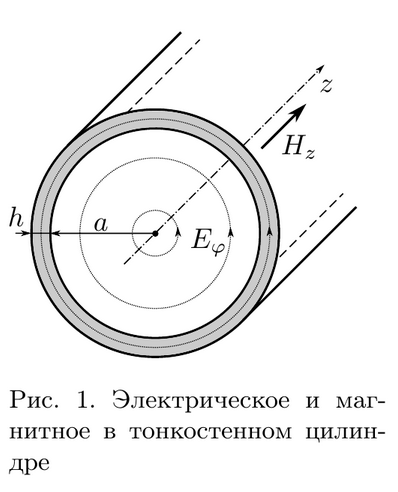
\includegraphics[width=4cm]{Screenshot_1.png}
	\label{pic:2}
\end{wrapfigure}

В работе изучается явление скин-эффекта в длинном медном тонкостенном цилиндре, помещенном в соленоид. Будем считать цилиндр достаточно длинным и пренебрегать краевыми эффектами, в этом приближении $H$ всюду направлено по оси симметрии системы, а $E$ - перпендикулярно радиусу. Будем считать, что эти поля колеблются по гармоническому закону с частотой задаваемой током в соленоиде:

\begin{equation}
	H_z = H(r)e^{iwt}
\end{equation}

\begin{equation}
	E = E(r)e^{iwt}
\end{equation}

Пусть радиус цилиндра $a$, толщина стенки $h << a$, тогда можно ограничиться одномерным решением задачи о скин-эффекте. Внутри цилиндра токи отсутствуют, поэтому поле однородно и $H(r) = H_1 = const$. Воспользуемся интегральным законом электромагнитной индукции и получим связь электрического и магнитных полей на внутренней границе цилиндра:

\begin{wrapfigure}{r}{4cm}
	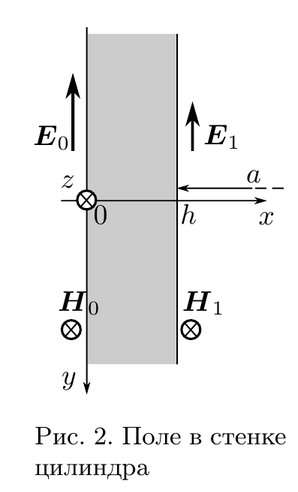
\includegraphics[width=4cm]{Screenshot_2.png}
	\label{pic:2}
\end{wrapfigure}

\begin{equation}
	E\cdot 2\pi r = -\mu_0\pi r^2 \cdot \frac{dH_z}{dt}
\end{equation}

\begin{equation}
	E_1 = -\frac{1}{2}iwa\mu_0 H_1
\end{equation}

Поле внутри стенки цилиндра будет описываться одномерным уравнением диффузии поля:

\begin{equation}
	\frac{d^2H}{dx^2} = iw\sigma\mu_0H
\end{equation}

Данное уравнение вместе с краевыми условиями $H_0$ и $H_1$ полностью определяет поля в стенке. Стоит отметить, что $H_0$ зависит только от тока в обмотке соленоида. Тогда:

\begin{equation}
	H(x) = Ae^{\alpha x} + Be^{-\alpha x}
\end{equation}

\begin{equation}
	\alpha = \sqrt{iw\sigma\mu_0} = \frac{1 + i}{\delta} = \frac{\sqrt{2}e^{i\frac{\pi}{4}}}{\delta}
\end{equation}

$\delta$ здесь - толщина скин слоя, на которой амплитуды полей спадают в $e$ раз. Первое граничное условие дает $A + B = H_0$, используя это можно преобразовать выражение(6):

\begin{equation}
	H(x) = H_0e^{-\alpha x} + 2Bsh(\alpha x)
\end{equation}

Далее, воспользовавшись законом Ампера в одномерном варианте $E(x) = \frac{1}{\sigma}\frac{\partial H}{\partial x}$, мы можем используя соотношения на $E_1$ и $H_1$, полученное ранее, исключить константу и в итоге получить:

\begin{equation}
	H_1 = \frac{H_0}{ch(\alpha h) + \frac{1}{2}\alpha a sh(\alpha h) }
\end{equation}

Далее следует рассмотреть предельные случаи:

1. Частота тока в соленоиде мала, $\delta >> h$, тогда:

\begin{equation}
	\frac{|H_1|}{|H_0|} = \frac{1}{\sqrt{1 + \frac{1}{4}(ah\sigma \mu_0 w)^2}}
\end{equation}

\begin{equation}
	tg(\psi) = \frac{ah}{\sigma^2}
\end{equation}

$\psi$ - разность фаз $H_1$ и $H_0$.

2. Частота тока в соленоиде высока, $\delta << h$, тогда:

\begin{equation}
	\frac{H_1}{H_0} = \frac{2\sqrt{2}\delta}{a}e^{-\frac{h}{\delta}}e^{-i(\frac{\pi}{4} + \frac{h}{\delta})}
\end{equation}

\begin{equation}
	\psi = \frac{\pi}{4} + h\sqrt{\frac{w\sigma \mu_0}{2}}
\end{equation}

Скин эффект также оказывает влияние на индуктивность катушки:

\begin{equation}
	\Phi = \Phi_{out} + \Phi_{in} = H_0S_0 + H_1S_1 = LI
\end{equation}

Учитывая независимость внешнего потока от частоты, можем записать:

\begin{equation}
	\L_{min} = \frac{\Phi_{out}}{I}
\end{equation}

Найдем соотноошение потоков:

\begin{equation}
	\Phi_{in} = H_1S_1 = \Phi_{out}\frac{S_1}{nS_0}
\end{equation}

Где n - отношение напряженности поля снаружи и внутри цилиндра. Максимальное поле достигается при $H_0 = H_1$, поэтому:

\begin{equation}
	\Phi_{max} = H_0(S_0 + S_1) = L_{max}I
\end{equation}

и тогда:

\begin{equation}
	\frac{S_1}{S_0} = \frac{L_{max} - L_{min}}{L_{min}}
\end{equation}

Используя (14) и (18), а также соотношения ранее:

\begin{equation}
	\frac{L_{max} - L}{L - L_{min}} = \pi^2a^2h^2\mu_0^2\sigma^2\nu^2
\end{equation}


 

\section{Экспериментальная установка}

\begin{wrapfigure}{r}{6.5cm}
	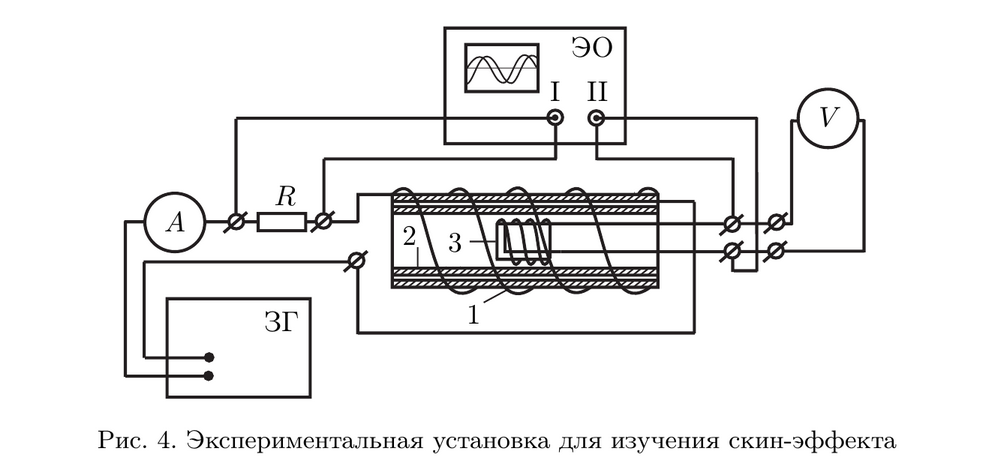
\includegraphics[width=6.5cm]{Screenshot_3.png}
\end{wrapfigure}


Схема экспериментальной установки для исследования проникновения переменного магнитного поля в медный полый цилиндр изображена на рис. 4. Переменное магнитное поле создаётся с помощью соленоида, намотанного на полый цилиндрический каркас 1 из поливинилхлорида, который подключается к генератору звуковой частоты. Внутри соленоида расположен медный цилиндрический экран 2. Для измерения маг-
нитного поля внутри экрана используется измерительная катушка 3. Необходимые параметры соленоида, экрана и измерительной катушки указаны на установке. Действующее значение переменного тока в цепи
соленоида измеряется амперметром А, а действующее значение напряжения на измерительной катушке измеряет вольтметр V. Для измерения сдвига фаз между током в цепи соленоида и напряжением на измерительной катушке используется двухканальный осциллограф. На вход одного канала подаётся напряжение с резистора R, которое пропорционально току, а на вход второго канала - напряжение с измерительной катушки.

Заметим некоторые соотношения, которые будет удобно измерять в ходе эксперимента:

Для напряжения на измерительной катушке, справедливо:

\begin{equation}
	U = -SN\frac{dB_1}{dt} = -iw\mu_0 SNH_1 e^{iwt}
\end{equation}

Тогда измереряемая вольтметром величина(усреднение по времени переменного напряжения):

\begin{equation}
	U = \frac{SNw}{\sqrt{2}}\mu_0|H_1|
\end{equation}

То есть:

\begin{equation}
	|H_1|\propto \frac{U}{\nu}
\end{equation}

При этом:

\begin{equation}
	|H_0|\propto I
\end{equation}

Тогда очевидно:

\begin{equation}
	\frac{|H_1|}{|H_0|} = const\cdot \frac{U}{\nu I}
\end{equation}

Константу из соотношения выше далее будем обозначать $\xi_0$.

Разность фаз магнитных полей на границе и в полости цилиндра в ходе эксперимента определяется с помощью осциллографа. Деления, за которые ток в обмотках, фиксирующийся через амперметр, проходит половину фазы, обозначается далее за $X$, а минимальное расстояние между нулями тока и напряжения в измерительной катушке внутри соленоида за $X_0$. Тогда очевидно:

\begin{equation}
	\psi = \frac{X_0}{X} \cdot \pi - \pi/2
\end{equation}

Вычитание $\pi / 2$ связанно с тем, что напряжение на катушке - это производная по времени поля внутри, что дает дополнительную прибавку к фазе $\pi / 2$. 


\section{Ход работы}

\subsection{Определение $\xi_0$ и $\sigma$ по низким частотам}

Сначала оценим частоту, на которой $\delta = h$, полагая $\sigma = 5\cdot10^{7}$ См/м, используя формулу (7):

\begin{equation}
	\nu = \frac{1}{\pi h^2\sigma \mu_0} \approx 2250 \text{ Гц}
\end{equation}

Так как все вычисления в обработке сводятся к использованию одних и тех же данных, представленных в различных частотных диапазонах, будет удобно свести все наблюдения в серию таблиц:

Далее 

\begin{table}[H]
	\centering
	\begin{tabular}{|c|c|c|c|c|c|c|c|c|c|c|}
		\hline
		$ \nu $, Гц   & 22.5   & 32.5   & 42.5   & 50   & 60   & 70   & 80   & 90 & 100 & 110 \\ \hline
		$ U $, В & 0.1555 & 0.2207 & 0.2817 & 0.3246 & 0.3776 & 0.4255 & 0.4686 & 0.5069 & 0.5409 & 0.5708\\ \hline
		$ I $, мА & 435.4 & 432.5 & 427.9 & 424.0 & 418.2 & 412.0 & 405.8 & 399.5 & 393.4 & 387.4 \\ \hline
		$ X $  & - & - & - & - & - & - & - & - & - & - \\ \hline
		$ X_0 $  & - & - & - & - & - & - & - & - & - & - \\ \hline
	\end{tabular}
	\caption{Результаты измерений до 0.5 $\nu_h$ - 1}
	\label{tab:my-table1}
\end{table}

\begin{table}[H]
	\centering
	\begin{tabular}{|c|c|c|c|c|c|c|c|c|c|c|c|}
		\hline
		$ \nu $, Гц   & 130   & 153   & 176   & 200   & 225   & 300 & 400 & 500 & 600 & 700 & 800 \\ \hline
		$ U $, В & 0.6202 & 0.6634 & 0.6957 & 0.7208 & 0.7402 & 0.7725 & 0.7870 & 0.7871 & 0.7801 & 0.7720 & 0.7581 \\ \hline
		$ I $, мА & 376.0 & 364.9 & 355.8 & 347.8 & 341.0 & 326.4 & 314.3 & 305.7 & 298.3 & 292.5 & 285.5 \\ \hline
		$ X $  & 1.4 & 2.4 & 2.2 & 2.1 & 1.8 & 3.9 & 2.8 & 1.9 & 4.4 & 3.7 & 3.2 \\ \hline
		$ X_0 $  & 1.8 & 3.2 & 2.8 & 2.5 & 2.2 & 3.3 & 2.4 & 2 & 4.2 & 3.6 & 3.1 \\ \hline
	\end{tabular}
	\caption{Результаты измерений до 0.5 $\nu_h$ - 2}
	\label{tab:my-table1}
\end{table}

\begin{table}[H]
	\centering
	\begin{tabular}{|c|c|c|c||c|}
		\hline
		$ \nu $, Гц   & 900   & 950   & 1000 & 1120 \\ \hline
		$ U $, В & 0.7439 & 0.735 & 0.7271 & 0.706 \\ \hline
		$ I $, мА & 278.5 & 275.0 & 271.5 & 263.0 \\ \hline
		$ X $  & 2.8 & 2.6 & 2.5 & 4.4  \\ \hline
		$ X_0 $  & 2.7 & 2.6 & 2.4 & 4.4 \\ \hline
	\end{tabular}
	\caption{Результаты измерений до 0.5 $\nu_h$ - 3}
	\label{tab:my-table1}
\end{table}

Построим по данным первых двух таблиц график $\frac{1}{\xi^2}$ от $\nu^2$ и используем точки от 22.5 до 400 Гц для линейной аппроксимации (далее наблюдаются серьезные отклонения от линейности зависимости). Погрешность для значений была взята как их супремум:



\begin{center}
	\begin{tikzpicture}
		\begin{axis}[
			title={График 1 \quad График зависимости $ \frac{1}{\xi^2}(\nu^2) $},
			xlabel={$ \nu^2 $, Гц $ ^2 $},
			ylabel={$\frac{1}{\xi^2}$},
			legend pos=south east,
			xmajorgrids=true,
			ymajorgrids=true,
			grid style=dashed,
			width = 520,
			height = 350,
			%xmin = 300,
			%xmax = 335,
			%ymin =40,
			%ymax =135,
			]
			\legend{ 
				Экспериментальные данные,
				Аппроксимация данных
			};
			\addplot [black, only marks, mark size = 2pt,
			error bars/.cd,
			x dir=both, x explicit,
			y dir=both, y explicit, 
			] table [x = T, y = sigma, y error plus = YError, y error minus = YError] {
				T	sigma       YError          
				506.25  3969    152
				1056.25	4056.3  152
				1806.25	4167.6  152
				2500    4265    152
				3600    4415.8  152
				4900    4594    152
				6400    4799.5  152
				8100    5031.2  152
				10000   5289.7  152
				12100   5573.6  152
				16900   6211.5  152
				23409   7082.4  152
				30976   8102.0  152
				40000   9313.0  152
				50625   10744.2 152
				90000   16067.4 152
				160000  25518.5 152
			};
		\addplot [blue, domain=0:160000, line width =3.2pt] {0.1349*x + 3926.4};
		\end{axis}
	\end{tikzpicture}
\end{center}

: 
\[ k = (0.1349 \pm 0.001). \]
\[ b = (3926.4 \pm 152). \]

По полученному значению элементарно рассчитаем $\xi_0$:

\begin{equation}
	\xi_0 = \sqrt{b} = 62.7 \pm 1.2
\end{equation}

и используя полученный коэффициент k и соотношение (10), получаем для $\sigma$:

\begin{equation}
	\sigma = \frac{\sqrt{k}}{\xi_0} \cdot \frac{1}{\pi ah\mu_0} \approx 4.71 \pm 0.3 \cdot 10^7 \text{ См/м}
\end{equation}


\subsection{Определение $\sigma$ фазовым методом, средние частоты}

Получим график зависимости $tg(\psi)$ от $\nu$ для частот от $0.05 \nu_h$ до $0.5 \nu_h$: 

\begin{center}
	\begin{tikzpicture}
		\begin{axis}[
			title={График 2 \quad График зависимости $ tg(\psi)(\nu) $},
			xlabel={$ \nu $, Гц},
			ylabel={$tg(\psi)$},
			legend pos=south east,
			xmajorgrids=true,
			ymajorgrids=true,
			grid style=dashed,
			width = 520,
			height = 350,
			%xmin = 300,
			%xmax = 335,
			%ymin =40,
			%ymax =135,
			]
			\legend{ 
				Экспериментальные данные,
				Уровень "бесконечность",
				Аппроксимация данных,
			};
			\addplot [black, only marks, mark size = 2pt,
			error bars/.cd,
			x dir=both, x explicit,
			y dir=both, y explicit, 
			] table [x = T, y = sigma, y error plus = YError, y error minus = YError] {
				T	sigma       YError          
				130    1.19    0.30    
				153	   1.0     0.50    
				176	   1.25    0.48    
				200    1.82    0.54      
				225    1.56    0.43    
				300    1.91    0.87    
				400    2.08    0.67    
				500    -6.0    1.16    
				600    6.96    3.10    
				700    11.75   4.37    
				800    10.15   3.27    
				900    8.88    2.50    
				950    0       0    
				1000  7.92     2.0    
				1120    0      0    
			};
			\addplot [red, domain=0:1120, line width =1.0pt]{0*x + 0};
			\addplot [blue, domain = 130:400, line width = 3.0pt]{0.0038*x + 0.69};
		\end{axis}
	\end{tikzpicture}
\end{center}

По разбросу и общему качеству данных можно заключить, что линейная аппроксимация здесь неуместна, но если все же для оценки допустить ее для первых 7 точек, больше всего напоминающих линейную зависимость, получим:

\begin{equation}
	k = 0.0038 \pm 0.0031
\end{equation}

И тогда из соотношений (7) и (11) получаем $\sigma$:

\begin{equation}
	\sigma = \frac{k}{ah\pi\mu_0} \approx 3.06 \pm 2.49 \cdot 10^7 \text{См/м} 
\end{equation}

\subsection{Определение $\sigma$ фазовым методом, высокие частоты}

Для данного метода используется диапазон частот от 0.5 $\nu_h$ до 15 $\nu_h$, данные перечислены в серии таблиц ниже:

\begin{table}[H]
	\centering
	\begin{tabular}{|c|c|c|c|c|c|c|c|c|c|c|}
		\hline
		$ \nu $, Гц   & 1405   & 1760 & 2210 & 2775 & 3480 & 4365 & 5477 & 6870 & 8620 & 10813 \\ \hline
		$ U $, В & 0.6537 & 0.5901 & 0.5175 & 0.4415 & 0.3676 & 0.2991 & 0.2380 & 0.1857 & 0.1417 & 0.1060\\ \hline
		$ I $, мА & 243.1 & 219.6 & 193.2 & 166.0 & 139.7 & 115.6 & 94.32 & 76.2 & 60.85 & 47.96 \\ \hline
		$ X $  & 3.4 & 2.7 & 4.3 & 3.3 & 2.5 & 1.9 & 3.5 & 2.6 & 1.9 & 2.7 \\ \hline
		$ X_0 $  & 3.5 & 2.8 & 4.6 & 3.6 & 2.9 & 2.3 & 4.5 & 3.6 & 2.8 & 4.6 \\ \hline
	\end{tabular}
	\caption{Результаты измерений от 0.5 $\nu_h$ до 15 $\nu_h$  - 1}
	\label{tab:my-table1}
\end{table}

\begin{table}[H]
	\centering
	\begin{tabular}{|c|c|c|c|c|c|}
		\hline
		$ \nu $, Гц   & 13565   & 17020 & 21350 & 26780 & 33600 \\ \hline
		$ U $, В & 0.0780 & 0.057 & 0.0427 & 0.0334 & 0.0280\\ \hline
		$ I $, мА & 37.05 & 27.63 & 19.25 & 11.4 & 4.02 \\ \hline
		$ X $  & 1.8 & 1.2 & 1.1 & 0.7 & 0.2 \\ \hline
		$ X_0 $  & 3.7 & 2.9 & 4.6 & 3.7 & 2.9 \\ \hline
	\end{tabular}
	\caption{Результаты измерений от 0.5 $\nu_h$ до 15 $\nu_h$  - 2}
	\label{tab:my-table1}
\end{table}

Построим график $\psi - \frac{\pi}{4}$ от $\sqrt{\nu}$:

\begin{center}
	\begin{tikzpicture}
		\begin{axis}[
			title={График 2 \quad График зависимости $\psi(\sqrt{\nu}) $},
			xlabel={$ \sqrt{\nu} $},
			ylabel={$\frac{\psi - \frac{\pi}{4}}{\pi}$},
			legend pos=south east,
			xmajorgrids=true,
			ymajorgrids=true,
			grid style=dashed,
			width = 520,
			height = 350,
			%xmin = 300,
			%xmax = 335,
			%ymin =40,
			%ymax =135,
			]
			\legend{ 
				Экспериментальные данные,
				Аппроксимация данных,
			};
			\addplot [black, only marks, mark size = 2pt,
			error bars/.cd,
			x dir=both, x explicit,
			y dir=both, y explicit, 
			] table [x = T, y = sigma, y error plus = YError, y error minus = YError] {
				T	sigma       YError          
				37.5    0.505    0.00013    
				42.0	0.506    0.00021    
				47.0	0.511    0.00024    
				52.7    0.514    0.00040      
				59.0    0.524    0.00086    
				66.1    0.530    0.00143    
				74.0    0.540    0.00097    
				82.9    0.551    0.00161    
				92.8    0.560    0.00250    
				104.0   0.581    0.00213    
				116.5   0.606    0.00357    
				130.5   0.625    0.00549    
				146.1   0.675    0.00498    
				163.6   0.690    0.00673    
				183.3   0.728    0.01003    
			};
			%\addplot [red, domain=0:1120, line width =1.0pt]{0*x + 0};
			\addplot [blue, domain = 130:190, line width = 3.0pt]{0.0019*x + 0.38};
		\end{axis}
	\end{tikzpicture}
\end{center}

Взяв последние 4 точки для линейной аппроксимации, получим:

\begin{equation}
	k = 0.0019 \pm 0.001
\end{equation}

Тогда $\sigma$ (из соотношения (13)):

\begin{equation}
	\sigma = (\frac{k\pi}{h\sqrt{\pi \mu_0}})^2 \approx 3.61\pm 0.44 \cdot 10^7 \text{ См/м}
\end{equation}

\subsection{Получение итоговой $\sigma$ и проверка теории об ослаблении полей}

Занесем в таблицу полученные коэффициенты проводимости:

\begin{table}[H]
	\centering
	\begin{tabular}{|c|c|c|c|}
		\hline
		$ \sigma $, $10^7$ См/м   & 4.71 $\pm 0.3$ & 3.06 $\pm 2.49$ & 3.61 $\pm 0.44$ \\ \hline
		№, способ   & 1  & 2 & 3 \\ \hline
	\end{tabular}
	\caption{Результаты рассчета $\sigma$}
	\label{tab:my-table1}
\end{table}

Первый результат, если судить по погрешности и качеству аппроксимации теоретических положений, сразу выделяется на фоне двух других. Используя полученное в первом способе $\xi_0$, рассчитаем коэффициент ослабления поля для всех измерений и получим график $\frac{H_1}{H_0}$ от $\nu$:

\begin{center}
	\begin{tikzpicture}
		\begin{axis}[
			title={График 2 \quad График зависимости $\frac{H_1}{H_0}(\ln{\nu}) $},
			xlabel={$ \ln{\nu} $},
			ylabel={$\frac{H_1}{H_0}$},
			legend pos=north east,
			xmajorgrids=true,
			ymajorgrids=true,
			grid style=dashed,
			width = 520,
			height = 350,
			%xmin = 300,
			%xmax = 335,
			%ymin =40,
			%ymax =135,
			]
			\legend{ 
				Экспериментальные данные,
				$\sigma$ 3 способа,
				$\sigma$ 1 способа,
			};
			\addplot [black, only marks, mark size = 2pt,
			error bars/.cd,
			x dir=both, x explicit,
			y dir=both, y explicit, 
			] table [x = T, y = sigma, y error plus = YError, y error minus = YError] {
				T						sigma       YError
			3.1135153092103742 0.9952380952380953 0.003034528852627153
			3.481240089335692 0.9844652734548689 0.0024296396430131192
			3.7495040759303713 0.9712324209889613 0.0021051211301746837
			3.912023005428146 0.9600198113207549 0.0019442412869348528
			4.0943445622221 0.9435485413677667 0.001789457047705763
			4.248495242049359 0.9250641470180305 0.0016747075788558427
			4.382026634673881 0.9050400443568261 0.0015842121819330038
			4.499809670330265 0.8839557780559033 0.0015102218517364016
			4.605170185988092 0.8620851550584648 0.001447037944914165
			4.700480365792417 0.8398451213216315 0.001392131263732335
			4.867534450455582 0.7955511456628477 0.0012997583061895796
			5.030437921392435 0.7450367814980199 0.001208201187952468
			5.170483995038151 0.6965798903878584 0.001126721258817063
			5.298317366548036 0.6497147786083957 0.0010513947363547955
			5.41610040220442 0.6048946236559141 0.0009805030758504225
			5.703782474656201 0.49464613970588234 0.0008081550853337661
			5.991464547107982 0.3924984091632199 0.0006485268400623924
			6.214608098422191 0.3228732090284593 0.0005398653533340845
			6.396929655216146 0.27328343949044587 0.0004633258148795047
			6.551080335043404 0.236407326007326 0.0004056899694526069
			6.684611727667927 0.2081123905429072 0.00036375114094642244
			6.802394763324311 0.18608629563135848 0.00033191735368353476
			6.856461984594587 0.1764 0.00031801148325358845
			6.907755278982137 0.16791591160220995 0.00030608624051972367
			7.02108396428914 0.15027906029331883 0.0002817675292202461
			7.247792581767846 0.12000096616801663 0.00024190589955894109
			7.473069088032197 0.09573002049180329 0.00021257279158849482
			7.700747794511798 0.0759938590820944 0.00019104839419083062
			7.928406026180535 0.06009345490068383 0.00017528154640263647
			8.15478757276852 0.04740972033668205 0.00016391666519055306
			8.381373468273702 0.037165661898476796 0.00015496394055260034
			8.608312784783722 0.028886702244547056 0.0001473264474642386
			8.834919385216395 0.022241687583811846 0.00014011610005098057
			9.061840363657739 0.016938289163379576 0.00013330211988886283
			9.288504392945537 0.012815868089464177 0.00012762400816412683
			9.515248225093032 0.009730925175082936 0.0001251196225478801
			9.742144402127366 0.007599796369092505 0.00013088382154919636
			9.96880701865677 0.006514285714285715 0.00016158951306304936
			10.195410619245164 0.006859596713965646 0.0002906034549550167
			10.422281345951296 0.012997512437810948 0.0015934155225007696
			};
		\addplot [red, only marks, mark size = 2pt,
		error bars/.cd,
		x dir=both, x explicit,
		y dir=both, y explicit, 
		] table [x = T, y = sigma, y error plus = YError, y error minus = YError] {
			T						sigma       YError
		3.1135153092103742 0.991831150503086 0
		3.481240089335692 0.9831029886272947 0
		3.7495040759303713 0.9714401816626221 0
		3.912023005428146 0.9608903488271511 0
		4.0943445622221 0.9446140957470106 0
		4.248495242049359 0.9260597298979459 0
		4.382026634673881 0.9055162257178208 0
		4.499809670330265 0.8832833893105745 0
		4.605170185988092 0.859662515153242 0
		4.700480365792417 0.8349481796578916 0
		4.867534450455582 0.7833445793964252 0
		5.030437921392435 0.7225401400241185 0
		5.170483995038151 0.6624548336674982 0
		5.298317366548036 0.6023569033450877 0
		5.41610040220442 0.5438472296913146 0
		5.703782474656201 0.3979377985729857 0
		5.991464547107982 0.2658453717541181 0
		6.214608098422191 0.1828674545309444 0
		6.396929655216146 0.12942026929262404 0
		6.551080335043404 0.09367955802765128 0
		6.684611727667927 0.06887327666608066 0
		6.802394763324311 0.05107103638557163 0
		6.856461984594587 0.044020398682463296 0
		6.907755278982137 0.037918507304403874 0
		7.02108396428914 0.026255786004001226 0
		7.247792581767846 0.009067629996455733 0
		7.473069088032197 -0.00206736070310733 0
		7.700747794511798 -0.009277365425469643 0
		7.928406026180535 -0.013779952201647456 0
		8.15478757276852 -0.016454019724793212 0
		8.381373468273702 -0.01787514262468859 0
		8.608312784783722 -0.018353623331252844 0
		8.834919385216395 -0.018044279723335718 0
		9.061840363657739 -0.017008497686647236 0
		9.288504392945537 -0.015282934043383052 0
		9.515248225093032 -0.012947118025423983 0
		9.742144402127366 -0.010189944128956184 0
		9.96880701865677 -0.00732145245861438 0
		10.195410619245164 -0.004685032652487981 0
		10.422281345951296 -0.002551967810460947 0
		};
		\addplot [blue, only marks, mark size = 2pt,
		error bars/.cd,
		x dir=both, x explicit,
		y dir=both, y explicit, 
		] table [x = T, y = sigma, y error plus = YError, y error minus = YError] {
			T						sigma       YError
			3.1135153092103742 0.9808558650755765 0
			3.481240089335692 0.960853464750505 0
			3.7495040759303713 0.9348285317845538 0
			3.912023005428146 0.9119524241496652 0
			4.0943445622221 0.877839334975471 0
			4.248495242049359 0.8406017211202917 0
			4.382026634673881 0.8012879107875045 0
			4.499809670330265 0.7608486722304304 0
			4.605170185988092 0.7201051956470438 0
			4.700480365792417 0.6797350918158642 0
			4.867534450455582 0.6021186780806851 0
			5.030437921392435 0.5206994183266047 0
			5.170483995038151 0.4492123199567288 0
			5.298317366548036 0.38521863673179535 0
			5.41610040220442 0.3290588935655731 0
			5.703782474656201 0.21023495609055895 0
			5.991464547107982 0.12286114438143612 0
			6.214608098422191 0.07552994376137419 0
			6.396929655216146 0.0476232726858382 0
			6.551080335043404 0.02997765091908598 0
			6.684611727667927 0.01818188377994179 0
			6.802394763324311 0.00993909968524122 0
			6.856461984594587 0.006726073944593476 0
			6.907755278982137 0.003969493107643403 0
			7.02108396428914 -0.001234442984143465 0
			7.247792581767846 -0.008724785457461129 0
			7.473069088032197 -0.013402205739184585 0
			7.700747794511798 -0.016248711509291792 0
			7.928406026180535 -0.01778345374760842 0
			8.15478757276852 -0.018343197685066197 0
			8.381373468273702 -0.01810735178031715 0
			8.608312784783722 -0.017141361016377796 0
			8.834919385216395 -0.015481845464164564 0
			9.061840363657739 -0.013197671142429852 0
			9.288504392945537 -0.010472459919523723 0
			9.515248225093032 -0.007598633966155825 0
			9.742144402127366 -0.004922180536405742 0
			9.96880701865677 -0.0027334646937310875 0
			10.195410619245164 -0.0011753495288490618 0
			10.422281345951296 -0.00024221031435657208 0
		};
			%\addplot [red, domain=0:1120, line width =1.0pt]{0*x + 0};
			
		\end{axis}
	\end{tikzpicture}
\end{center}


\section{Обсуждение результатов и выводы}

В ходе работы нами было использовано три метода для определения проводимости меди по скин-эффекту, косвенно в ней наблюдающемся: по соотношению амплитуд полей на низких частотах и по фазам на средних и высоких частотах. Первый и третий методы показывали в ходе эксперимента хорошее качественное совпадение с теорией, в отличие от второго, в котором ситуация кардинально противоположная. Проводимость, полученная в первом методе, хорошо совпадает с табличными значениями проводимости меди, учитывая примеси в ней, но построение графиков $\frac{H_1}{H_0}$ показало, что теория описала данные качественно, но не количественно. Результаты опытов, по нашему мнению, могут быть объяснены следующими положениями:

1. Использование в качестве теоретической основы упрощенного решения скин-эффекта для одномерного случая - это ведет к переоценке второй производной на высоких частотах и вследствии к занижению поля внутри цилинлра.

2. Предположение о стационарности полей может быть неккоретно на высоких частотах, когда характерные размеры системы уже не соответствуют характерной скорости распространения колебаний в системе.

3. Неточность определения фаз по нулям напряжений на изм. катушке и резисторе, особенно проявляющуюся при приближении разности фаз к $\pi$/2 и следственно совпадению фаз на осциллографе.

4. Качественное расхождение на средних частотах может быть связано с "переходом" решения между областями аппроксимации. Учитывая, что "опорная частота" была вычислена по оценке проводимости, границы перехода могли быть определены неточно.

В таких условиях, мы можем утверждать следущее: теория в одномерном приближении описывает наблюдения качественно, о качестве количественного описания судить сложно.

\section{Рекоммендации по установке}

Мы считаем нелишними следующие корректировки по данной работе:

1. Использовать альтернативный метод определения разности фаз, оправдавший себя в ранних работах - по фазовым диаграмам(используя осциллограф в режиме одного из сигналов поданного на временную развертку) для более высокой точности, либо использовать электронный осциллограф, на котором можно крайне точно определять нужные величины.

2. По первым рассчетам $\sigma$ корректировать "опорную частоту"

\end{document}